Enabling Lazy Shadowing for resiliency in extreme-scale computing 
brings about a number of challenges and design decisions that need to be addressed, including the applicability of this concept to a large number of 
tasks executing in parallel, the effective way to control shadows' execution rates, and the runtime mechanisms and 
communications support to ensure efficient coordination between a 
main and its shadow.
Taking into consideration the main characteristics of compute-intensive and highly-scalable applications, we design two novel techniques, referred to as {\it shadow collocation} and {\it shadow leaping}, in order to achieve high-tolerance to failure while minimizing delay and energy consumption. In the following, we first introduce the execution and communication model of the targeted applications. We then describe the dynamics of Lazy Shadowing with shadow collocation and shadow leaping. Lastly, we discuss important aspects of its implementation. 
%In the following, we first introduce the basic Lazy Shadowing resilience model. We then %focus on resilience in extreme-scale computing environments, where a large number of %communicating tasks execute in parallel to complete a job. 
%To achieve high tolerance to failure and reduce energy consumption in these environments, we %propose \emph{leaping shadows}, an instance of Lazy Shadowing. The main property of the %leaping shadows resilience model is its ability to sustain forward progress in the presence %of failures.
%. referred to as \emph{leaping shadows}, 
%a technique referred to as \emph{shadowed set rejuvenation} to reduce application failure probability, and 
%\emph{leaping shadows}, 
%as an 
%efficient, forward-progress preserving model to achieve high tolerance to failure, while reducing energy consumption, in these environments. 

 %We also discuss the runtime design issues
%related to enabling runtime support to efficiently achieve 
%the expected levels of resilience in extreme-scale systems. 

%This is to test referring Subsection \ref{frame_single}.



%\subsection{Application characteristics}
%\label{frame_app}
%%\subsection{Computational Model and Assumptions}
We consider the class of tightly-coupled and strongly scaled applications, executing on a large scale computing infrastructure of $N$ cores~\cite{doe_ascr_exascale_2011}. In this framework, the term core represents the unit of computing resource allocation (e.g., a
CPU core, a multi-core CPU, or a cluster node)~\cite{casanova_inria_2012}. This makes our framework agnostic to the granularity of the resource allocation unit.
%The focus of our model is a tightly-coupled and strongly scaling application, which executes on a large-scale platform
%composed of $N$ cores.
%We consider the execution of a tightly-coupled and strongly scaling application, or job, on a large-scale platform
%composed of $N$ cores. The application is tightly-coupled because this is typical in the HPC applications, and strong scaling because weak-scaling applications are not expected to suit for extreme-scale computing of which the cpu/memory imbalance would further increase~\cite{doe_ascr_exascale_2011}. Similar to \cite{casanova_inria_2012}, we use the term core to indicate unit of computing resource allocation (e.g., a
%CPU core, a multi-core CPU, or a cluster node), so that our work is agnostic to the granularity
%of the platform. 
%We assume that a standard checkpointing and roll-back recovery is performed at the
%system level. At most on application process (replica) runs on one core.


The application requires $W$ units of work, and can be split arbitrarily into a set of tasks.
Barriers are used as a method of synchronization among different tasks. Assuming $M \le N$ cores are assigned to the application, the failure-free completion time of the application is $w = W/M$. However, when a core fails, the whole execution will be suspended at the next barrier until recovery is complete. 

%The job can execute on any number $M \le N$ cores. The job is strong scaling so that the time required for a failure-free execution on $M$ cores is $w = W/M$.

%Cores are subject to failures. In most cases, we do not distinguish between soft and hard failures, with the understanding that soft failures are handled via software rejuvenation (i.e., rebooting \cite{466961}) and that hard failures are handled by the replacement of the failed component with a spare, which is a commonplace approach in production systems. For simplicity, we adopt the fail-stop fault model, where a core stops execution once a failure occurs and the failure can be detected by other cores \cite{gartner_faults_1999,cristian_comm_1991}. Since we consider tightly coupled parallel jobs, all $M$ cores operate synchronously. When a core fails, the whole execution is suspended until the failure is recovered. We assume that core failures are independent and identically distributed (i.i.d.). In the real world, instead, failures are bound to be correlated. Obtaining theoretical results for non-i.i.d. failures is beyond the scope of this work. But note that one cause of correlation is the hierarchical structure of computing platforms (each rack comprises compute nodes, each compute node comprises processors, and each processor comprises cores), which leads to simultaneous failures of a group of cores. Our work applies to such failures since a group of failures can be treated as multiple individual failures that happen at the same time and their recovery can be carried out in parallel.

Cores are subject to failures. In our model, we do not distinguish between soft and hard failures. We further assume that soft failures are handled via software rejuvenation (i.e., rebooting \cite{466961}), while hard failures are handled by replacing the failed components with spares. We adopt the fail-stop fault model, whereby a core stops executing upon failure and failures are detected by other non-failing cores \cite{gartner_faults_1999,cristian_comm_1991}. When a core fails, the whole execution is suspended until recovery is complete. 

%%%%%%%%%%%%%%%%%%%%%%%%%%%%%%rethinking%%%%%%%%%%%%%%%%%%%%%%
We assume that core failures are independent and identically distributed (i.i.d.). In the real world, instead, failures are bound to be correlated. Obtaining theoretical results for non-i.i.d. failures is beyond the scope of this work. But note that one cause of correlation is the hierarchical structure of computing platforms (each rack comprises compute nodes, each compute node comprises processors, and each processor comprises cores), which leads to simultaneous failures of a group of cores. Our work applies to such failures since a group of failures can be treated as multiple individual failures that happen at the same time and their recovery can be carried out in parallel.

%Since we consider tightly coupled parallel jobs, all q cores operate syn- chronously. These cores execute the same amount of work W(q) in parallel, chunk by chunk. The total time (on one core) to execute a chunk of dura- tion, or size, ω and then checkpointing it, is ω + C(q)

%\subsection{Leaping Shadows}



%%%%%%%%%%%%%%%%%%%%%%%%%%%%%%%%%%%%%%%%%%%%%%%%%%%%%%%%%%%%%%%%%%%%%%%%%%%%%%%%%%

%%We consider the class of strongly-scaled applications, and use $W$ to denote the size of an application workload~\cite{doe_ascr_exascale_2011}. The workload is split  arbitrarily into a set of $N$ tasks, whose synchronization is achieved using barriers. Assuming that each task is assigned to execute on a core at a maximum speed $\sigma=1$, the failure-free completion time of the application is $w = W/N$. 
Let $M_i$ denote the main process executing the $i^{th}$ task $T_i$, and $S_i$ its associated shadow.
When a failure occurs, the non-failing tasks continue executing until they reach the synchronization barrier. The tasks remain suspended until the shadow associated with the failing task reaches its synchronization barrier.


failure recovery is achieved.  To reduce time to recovery,  we run M shadows simulataneously with the main processes. 
%According to the computational model in Section~\ref{sec:com_model}, an application's workload is split into $M$ parallel tasks where each task is associated with a main process and a shadow.

 The execution of the application can be carried out by simultaneously running all main and shadow processes 
on %$2M$ cores, whereby the main processes execute at the maximum rate while the associated shadows execute at a fraction, $\sigma_s$, of the 
%maximum rate using DVFS. 
%To simultaneously run all the main and shadow processes,
%ne may choose to use $2M$ cores, with $M$ executing the main tasks at the maximum rate and $M$ \emph{lazily} executing the shadows at a fraction, $\sigma_s$, of the 
%maximum rate using DVFS.  
%An alternative method is to use 
$M+S$ cores, where $M$ is a multiple of $S$ and $M+S=N$, all executing at the maximum rate. $M$ of these cores are allocated to the main processes while the remaining $S$ cores are shared among their associated shadows. Based on this method, each main process is allocated one core, while $\alpha=M/S$ shadows are collocated on a single core. $\alpha$ is referred to as the main to shadow ratio.
For example, if $M=9$ and $S=3$, then the 9 shadows execute on 3 cores, with every $\alpha=3$ shadows executing on a core (Figure~\ref{fig:sc_mapping}).
%only $M+S$ cores can be used, whereby the main processes execute on the $M$ cores. And the $M$ shadows are divided into $S$ clusters with of $M/S$ shadows are colocated on a single core, operating at the maximum rate.
%where $M$ is a multiple of $S$, and collocate $M/S$ shadows on each of the $S$ cores, while executing all the cores at the maximum speed. 
%We use $\alpha$ to denote the main to shadow allocation ratio. %, and for simplicity, we assume the maximum execution rate of a core is 1. %Ignoring the overhead of context switching, the two alternatives lead to the same expected execution time, but different power and energy consumption. Specifically, the $2M$-cores scheme consumes more static but less dynamic power/energy than the $M+S$ cores alternative. The ratio between the system static and dynamic power consumption determines which alternative overall consumes less power/energy. 

%In the rest of the paper, we will focus on 
%shadow collocation as the meain the rest of our discussion 
%of the main ideas, concepts and system design. We will assume that all cores in the system execute at maximum speed, with every $\alpha=M/S$ shadows collocated on a core. 
%In HPC, throughput consideration requires that the rate of the main task, $\sigma_m$, and the shadow after failure, $\sigma_a$, be set to the maximum. The execution rate of the shadow before failure, $\sigma_b$, however, may still be used to manage the trade-offs between completion time and energy consumption. Smaller $\sigma_b$ corresponds to lazier shadowing of the main process. 
%In terms of execution rates, this can be expressed as $\sigma_m=\sigma_a=1$ and $\sigma_s \le 1$. 
  
Collocation of $\alpha$ shadows on a core has an important ramification with respect to the resilience of the system. Specifically, to speed up a shadow 
of a failed main to the maximum rate, all other collocated shadows must be terminated. Consequently, a second failure in any of the mains of the terminated shadows cannot be tolerated. In other words, the $M+S$ cores are grouped into $S$ sets, which we call \emph{shadowed sets}, each containing $\alpha+1$ cores with $\alpha$ mains executing on $\alpha$ cores (referred to as main cores) and their corresponding $\alpha$ shadows collocated on one core (referred to as shadow core). Each shadowed set can tolerate a failure in any of its cores, since failure of a main core would be recovered by the shadow core and failure of the shadow core will not affect any mains. After the first failure in a shadowed set, the set is called \emph{vulnerable} because it cannot tolerate another failure. %In the following subsection, we will discuss a rejuvenation scheme that deals with vulnerable shadowed sets.

\begin{figure}[!t]
	\begin{center}
		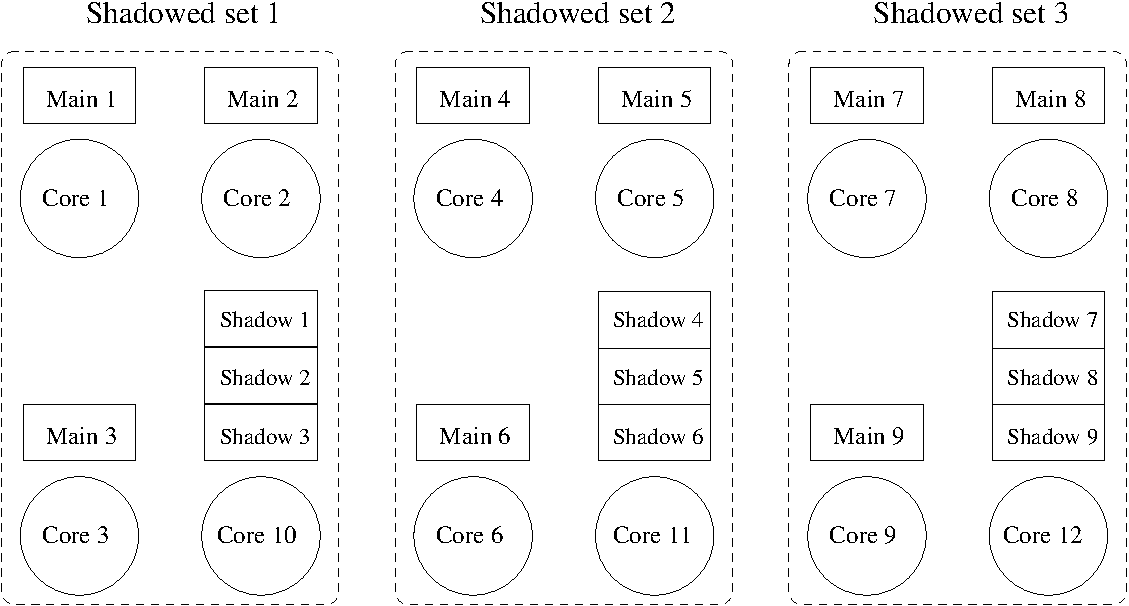
\includegraphics[width=\columnwidth]{Figures/sc_mapping.pdf}
	\end{center}
	\vskip -0.25in 
	\caption{An example of 3 shadowed sets with $\alpha=3$.}
	\label{fig:sc_mapping}
\end{figure}

%Lazy Shadowing provides the basis for the design of efficient energy- and power-aware fault-tolerance solutions for extreme-scale computing environments. %The resulting model, referred to as {\it leaping shadows}, 


%Lazy shadowing provides the basis for the design of efficient energy- and power-aware fault-tolerance solution for extreme-scale computing environments. The resulting model, referred to as {\it leaping shadows}, takes into consideration the main characteristics of compute-intensive and highly-scalable applications to achieve high-tolerance to failure, while minimizing energy consumption. In the following, we first introduce the execution and communication model of the targeted applications. We then describe the dynamics of the {\it leaping shadows} resilience model. Lastly, we discuss important aspects of its implementation. 
\subsection {Application model}
\label{sec:app_model}

We consider the class of compute-intensive and strongly-scaled applications, executing on a large-scale multi-core computing infrastructure~\cite{doe_ascr_exascale_2011}. %Communication between cores is achieved using low-latency, high-bandwidth interconnect networks, such as Infiniband. 
We use $W$ to denote the size of an application workload, and assume that the workload is split into a set of tasks, $T$, which execute in parallel. % and are synchronized using barriers. 
Assuming the maximum execution rate is $\sigma_{max}=1$, the failure-free completion time of the application is $W/|T|$. 
Given the prominence of MPI in HPC environments, we assume message passing as the communication mechanism between tasks. %Based on this model, each pair of communicating tasks is associated with a logical first-in-first-out (FIFO) channel, which guarantees ordered delivery of messages.
The execution is composed of a set of iterations separated by synchronization barriers. 
%The execution is divided into a set of phases by synchronization barriers. 


 %If a failure occurs, however, the non-failing tasks would become idle when they reach their synchronization barrier. These tasks remain idle until the failure recovery is complete. 
%resulting in performance hiccups~\cite{muller2010}, especially for tightly-coupled applications. 


\subsection{Shadow collocation}

%The execution of an application can be carried out by simultaneously running all tasks, each with a pair of main and shadow processes. Let $m_i$ denote the main process executing the $i^{th}$ task $\tau_i$, and $s_i$ its associated shadow.
%There are multiple ways to control the execution rates of the processes. The most straightforward solution is to allocate a dedicated core for each process while using 
%Dynamic Voltage and Frequency Scaling (DVFS) is a commonly used power management technique 
We use the term core to represent the resource allocation unit (e.g., a
CPU core, a multi-core CPU, or a cluster node), so that our algorithm is agnostic to the
granularity of the hardware platform~\cite{casanova_inria_2012}. Each main process executes on one core exclusively to achieve maximum throughput.  
To control the shadow's execution rate, Dynamic Voltage and Frequency Scaling (DVFS) can be applied while each shadow also uses one core exclusively~\cite{mills_2014_icnc,cui_en7085151,cui_2014_closer}. 
The effectiveness of DVFS, however, may be markedly 
limited by the granularity of voltage control, the number of frequencies available, and the negative effects on 
reliability~\cite{chandra2008defect}.
%reduced in computational platforms that exhibit saturation of the processor clock frequencies, large static power consumption, or small power dynamic range. 
 %Given our focus on extreme-scale, multi-core computing infrastructure, we will use collocation for execution rate control.  
%Recent development in processor and memory technology which results in the saturation of the processor clock frequencies, larger static power consumption, and smaller power dynamic range can markedly reduce the effectiveness of DVFS

 %to tune the frequency of the core. An alternative is to collocate multiple processes on a core, which runs at the maximum rate, and execute the processes in a time sharing manner. In the rest of this paper, we will focus on the idea of collocation in the discussion of applying Lazy Shadowing to HPC applications.  

An alternative is to collocate multiple shadows on a single core while keeping the core at maximum rate. Time sharing can then be used to achieve the desired execution rates.
To execute an application of $M$ tasks, $N=M+S$ cores are required, where $M$ is a multiple of $S$. Each main is allocated one core (referred to as \textit{main core}), while $\alpha=M/S$ (referred to as \textit{collocation ratio}) shadows are collocated on a core (\textit{shadow core}). 
The $N$ cores are grouped into $S$ sets, each of which we call a \textit{shadowed set}. Each shadowed set contains $\alpha$ main cores and 1 shadow core.
% $\alpha$ is referred to as shadowing ratio. For example, if $M=9$ and $S=3$, then the 9 shadows share 3 cores, with every $\alpha=3$ shadows collocated on each core, as shown in Figure~\ref{fig:sc_mapping}.
This is illustrated in Figure~\ref{fig:sc_mapping}.  

Collocation has an important ramification with respect to the resilience of the system. Specifically, 
one failure can be tolerated in each shadowed set. If a shadow core fails, all the shadows in the 
shadowed set will be lost without interrupting the execution of the mains. 
On the other hand, if a main core fails, the associated shadow will be promoted to a new main, and all 
the other collocated shadows will be terminated to speed up the new main.
%to speed up a shadow 
%of a failed main to the maximum rate, all other collocated shadows must be terminated. 
Consequently, a failure, either in main or shadow core, will result in losing all the shadows in the shadowed set, thereby losing the tolerance to any other failures. %After the first failure, a shadowed set becomes \emph{vulnerable}\footnote{Rejuvenation techniques, such as restarting the lost shadows from the state of current mains on spare cores, can be used to eliminate vulnerability.}. 
Quantitative study of this effect using probability theory is presented in Section~\ref{anal_app_fail}. %, this should not be a concern as the provided reliability is more than enough.
 
\begin{figure}[!t]
  \begin{center}
    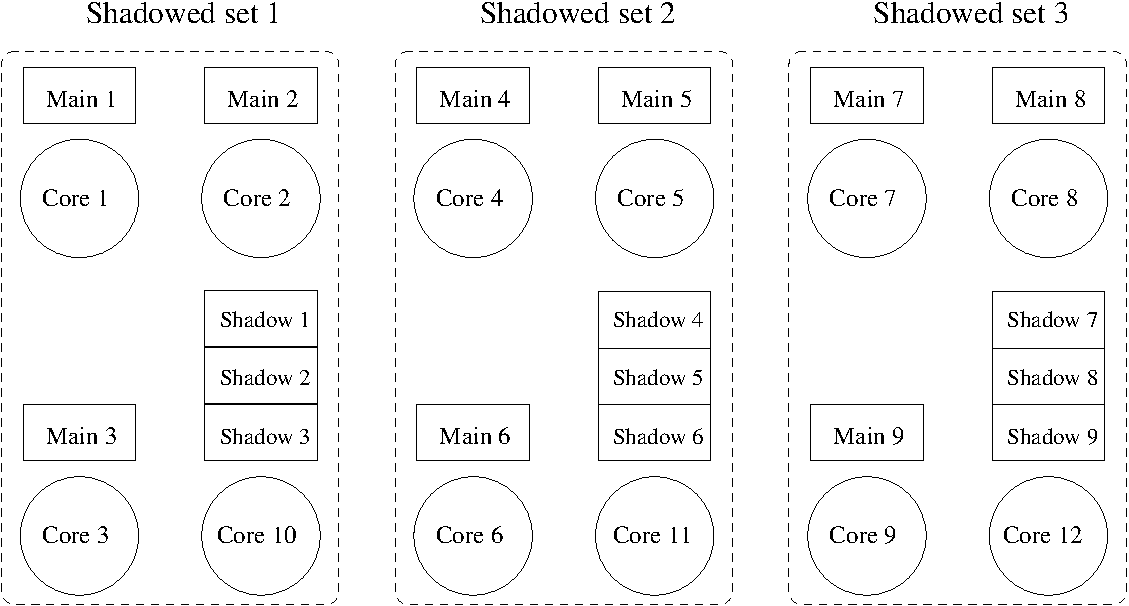
\includegraphics[width=\columnwidth]{Figures/sc_mapping.pdf}
  \end{center}
  %\vskip -0.25in 
  \caption{An example of collocation. $N=12$, $M=9$, $S=3$.}
  \label{fig:sc_mapping}
\end{figure}




\subsection {Shadow leaping}
\label{sec:leaping_shadows}

As the shadows execute at a lower rate, failures will incur delay for recovery. This problem deteriorates as dependencies incurred by messages and synchronization barriers would propagate the delay of one task to others.  
%The main objective of shadow leaping shadows is to minimize the delay induced by failures, 
%mitigate the impact of performance hiccups, 
Fortunately, slowing down the shadows provides an opportunity for the shadows to benefit from the faster execution of their mains. By copying the state of each main to its shadow, which is similar to the process of storing a checkpoint in a buddy in \cite{zheng_2004_ftccharm}, forward progress is achieved for the shadows with minimized time and energy. This technique, referred to as \textit{shadow leaping}, effectively limits the distance between main and shadow in progress. 
%, which simultaneously reduces the recovery time for failures. 
As a result, the recovery time after a failure, which depends on the distance between the failing main 
and its shadow, is also reduced. 
More importantly, %shadow leaping does not necessarily require the stopping of all the mains during normal execution, which will incur extra overhead even for failure-free execution. 
%Instead, 
we opportunistically overlap shadow leaping with failure recovery to avoid extra overhead. 
%and ensure forward progress by opportunistically rolling-forward the shadows during failure recovery. In Section~\ref{anal_time}, we will show that the delay is well bounded even for tightly-coupled applications.

%In the absence of failure, the behavior of a main  and its leaping shadow is identical to the behavior depicted in Figure \ref{fig:sync}. 
Assuming a failure occurrence at time $t_f$, Figure~\ref{fig:leap} shows the concept of shadow leaping. 
%Figure~\ref{fig:jump1} depicts the execution dynamics of the failing main and its associated shadow. 
Upon failure of a main process, its associated shadow speeds up to minimize the impact of failure recovery on the other tasks' progress, as illustrated in Figure~\ref{fig:jump1}. 
%Figure~\ref{fig:jump2} illustrates the behavior of the remaining main processes and their associated shadows. 
At the same time, as shown in Figure~\ref{fig:jump2}, the remaining main processes continue execution until the barrier at $W_{syn}$, and then become idle until $t_r$. %, when the shadow of the failed main also reaches the barrier. %It is worth noting that, given the tightly-coupled and strongly-scaled nature of the application, synchronization points occur frequently. Consequently, the time between synchronization points is very small relative to the total execution time of the application. Therefore, if one main, $m_i$, fails at 
%time $t_f$, the remaining main processes will reach their synchronization point, shortly after the failure, specifically at at time $t_{sync} = t_f +\epsilon$, 
%where $\epsilon \approxeq 0$. 
Shadow leaping opportunistically takes advantage of this idle time to {\it leap forward} the shadows by copying state from their mains, so that  
all processes, including shadows, can resume execution from a consistent point afterwards. %This process continues until the completion of all tasks. 
Shadow leaping increases the shadow's rate of progress, at a minimal energy cost. Consequently, it reduces significantly the likelihood of a shadow falling excessively behind, thereby ensuring fast recovery while minimizing energy consumption.



\begin{figure}[!t]
	\begin{center}
        \subfigure[Faulty task behavior.]
		{
			\label{fig:jump1}
			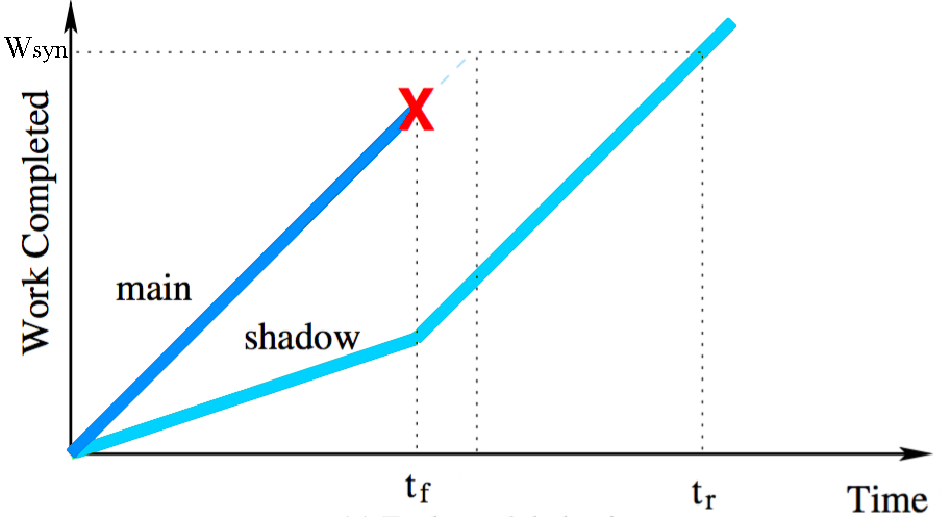
\includegraphics[width=0.7\columnwidth]{Figures/jump1.pdf}
		}
		\subfigure[Non-faulty task behavior.]
		{
			\label{fig:jump2}
			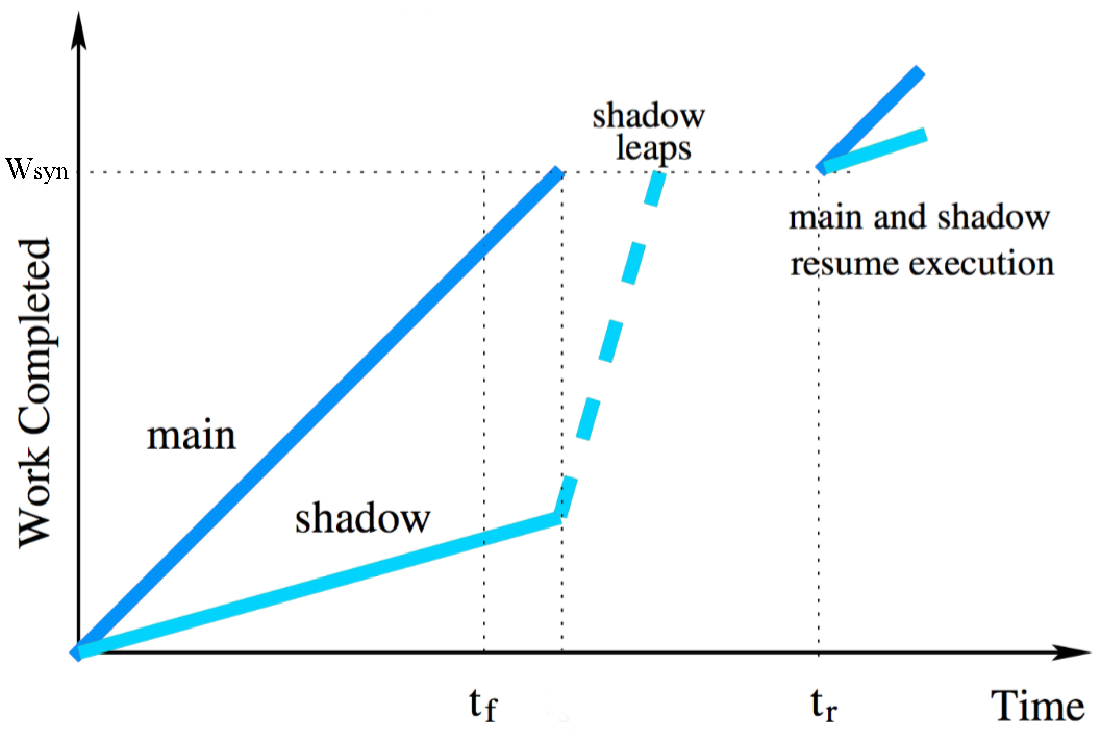
\includegraphics[width=0.7\columnwidth]{Figures/jump2.pdf}
		}
	\end{center}
	%\vskip -0.25in
	\caption{The illustration of shadow leaping.}
	\label{fig:leap}
\end{figure}

%Collocation is used to control the execution rates. To execute an application with $M$ tasks, $N=M+S$ cores are required, where $M$ is a multiple of $S$. Each main process is allocated one core (referred to as main core), while $\alpha=M/S$ shadows are collocated on a core (shadow core). 
%The $N$ cores are grouped into $S$ sets, which we call \emph{shadowed sets}, each containing $\alpha$ main cores and 1 shadow core.
%% $\alpha$ is referred to as shadowing ratio. For example, if $M=9$ and $S=3$, then the 9 shadows share 3 cores, with every $\alpha=3$ shadows collocated on each core, as shown in Figure~\ref{fig:sc_mapping}.
%This is illustrated in Figure~\ref{fig:sc_mapping}.  
%Collocation has an important ramification with respect to the resilience of the system. Specifically, 
%one failure can be tolerated in each shadowed set. If a shadow core fails, the main processes can continue
%execution, but will have no shadows any more. On the other hand, 
%to speed up a shadow 
%of a failed main to the maximum rate, all other collocated shadows must be terminated. Consequently, a second failure in any of the mains in the shadowed set cannot be tolerated. After the first failure, a shadowed set becomes \emph{vulnerable}\footnote{Rejuvenation techniques, such as restarting the lost shadows from the state of current mains on spare cores, can be used to eliminate vulnerability.}. 
%
%\begin{figure}[!t]
%  \begin{center}
%    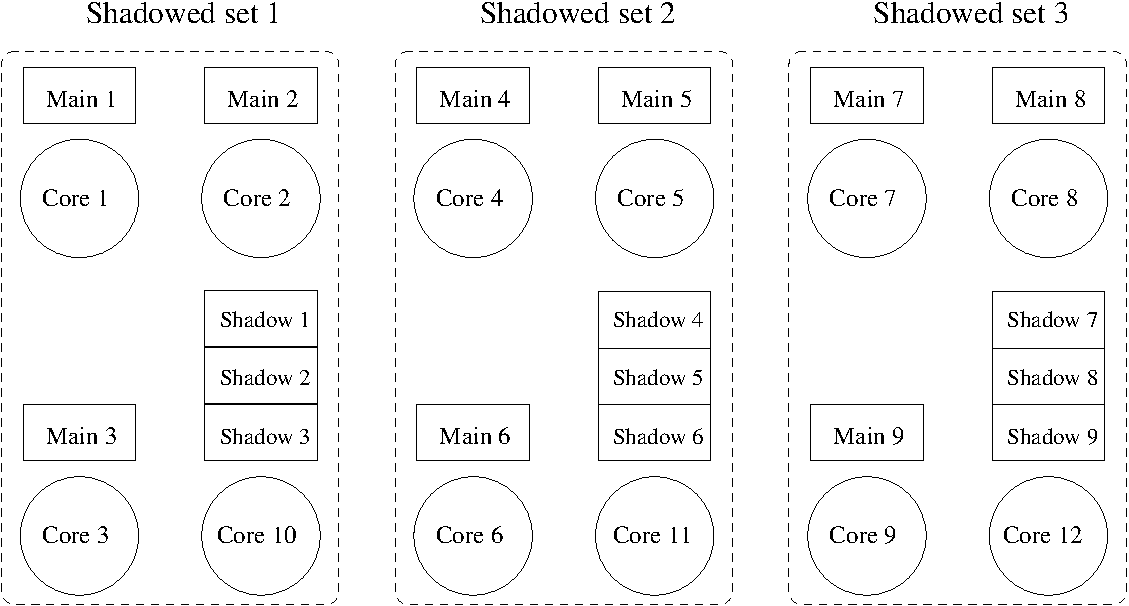
\includegraphics[width=\columnwidth]{Figures/sc_mapping.pdf}
%  \end{center}
%  %\vskip -0.25in 
%  \caption{An example of collocation. $N=12$, $M=9$, $S=3$.}
%  \label{fig:sc_mapping}
%\end{figure}

%Collocation also increases memory requirement. However, this is not intrinsic to Lazy Shadowing, as checkpointing/restart also requires additional memory capacity. We acknowledge the fact that compute kernels in existing HPC environments were simplified significantly by placing a number of restrictions, including eliminating virtual paging and limiting support for OS (Linux) to a handful of system calls. It became clear, however, that strategies designed to work around the capabilities of the hardware cannot scale to extreme-scale computing. Consequently, the research focus has been on new paradigms focused on co-design of hardware with system software to leverage the advantages associated with dynamic, asynchronous mechanisms, such as demand paging and cache tuning, against the design principles and choices of current HPC systems. Support of efficient demand paging, through co-design, is particularly critical as it is expected that the data of future exascale applications may not fit entirely in memory. %Finally, in comparison to checkpointing/restart and process replication, Lazy Shadowiing has the capability to control memory usage, based on the nature of failure and existing memory capacity, albeit at a loss of performance. 



\begin{algorithm}[t]
  \SetKwInOut{Input}{input}
  \SetKwInOut{Output}{output}
  \caption{Lazy Shadowing}
  %\Input{$W, M, S$}
  \Input{$M, S$}
  \Output{Application execution status}
  \BlankLine
  %split $W$ into $M$ tasks\; \nllabel{line:split} 
  %assign $M$ tasks to $S$ shadowed sets\; \nllabel{line:cluster} 
  %$T_l \leftarrow T+t_{now}$\;%, $C_{vul} \gets 0$
  %start $m_i$ and $s_i$ for each $task_i$\;
  start $M$ pairs of main and shadow\;
  map processes to cores\;
    \While{execution not done}
    {
  %      \If{failure detected in $ss_j$} %\nllabel{line:if_start_1} 
        \If{failure detected}
        {
            \nllabel{line:if_start_1} 
            %\eIf{$ss_j$ is vulnerable}
            \eIf{shadowed set is vulnerable}
            {
                notify ``Application fatal failure"\;
                %terminate all mains and shadows\;
                %repair all failures\;
                restart execution\; %\Comment{re-execution}
            }
            {
                mark the shadowed set as vulnerable\;
                %\State $C_{vul} \gets C_{vul} + 1$
                %\If{$C_{vul} == V$}
                %    \State perform shadowed set rejuvenation   
                %\EndIf 
                \If{failure happened to a main} 
                {
                    promote its shadow to new main\;
                    triggers shadow leaping\; %failure induced shadow leaping
                    %$T_l \leftarrow T+t_{now}$\;
                }
            }
        }  
        \nllabel{line:if_end_1}
        %\If{$t_{now} \ge T_l$} %
        %{
        %    \nllabel{line:if_start_2} 
        %    perform shadow leaping\;
        %    $T_l \leftarrow T+t_{now}$\;
        %    \nllabel{line:if_end_2}
        %} % 
        %\nllabel{line:if_end_2}
    }
    output ``Application completes"\;
  \label{al:ls}
\end{algorithm}

%The steps of applying Lazy Shadowing with leaping shadows are depicted in Algorithm 1.
We summarize the integration of shadow collocation and shadow leaping with basic shadowing in Algorithm 1.
User needs to specify $M$ for the number of parallel tasks, and $S$ for the number of shadow cores. These two parameters jointly determine the collocation ratio $\alpha=M/S$. The execution starts by simultaneously launching $2M$ processes, of which one main is associated with one shadow for each task (line 1). 
All processes are then grouped into $S$ shadowed sets. Accordingly, the processes are mapped to cores so that each shadowed set has $\alpha$ cores for $\alpha$ mains and 1 core for all the associated shadows (line 2). 
%To use $M+S$ cores to execute an application, the total workload is split into $M$ parallel tasks (line~\ref{line:split}), %, which are executed simultaneously by $M$ main processes and $M$ shadow processes. 
% which are then assigned to $S$ shadowed sets, each with $\alpha=M/S$ cores for $\alpha$ main processes and 1 core for all the associated shadow processes (line 2).  
%The $M$ shadows are then clustered into $S$ groups, each containing $\alpha=M/S$ shadows. 
%The execution starts by simultaneously running all the main and shadow processes (line 3).
During the execution,
the system runs a failure monitor (e.g., by using heartbeat protocol~\cite{1004595}) that triggers corresponding actions when a failure is detected (line~\ref{line:if_start_1} to~\ref{line:if_end_1}). %A failure may trigger different actions, depending on its type and precedence with respect to other failures.  A shadowed set becomes {\it vulnerable} after the occurrence of the first failure in the set. 
A failure occurring in a vulnerable shadowed set results in an application fatal failure %. In response, the system terminates all running 
%processes, initiates a recovery phase, either by rebooting or replacing failing cores,  and restarts execution (line 8 to 10). %(this assumes that checkpointing is not used). 
 and forces a rollback (line 6 and 7).
On the other hand, failure in a non-vulnerable shadowed set
can be tolerated while making the target shadowed set vulnerable (line 9). In this case, failure of a main need to be treated differently from failure of a shadow. While a failure of shadow 
does not impact the normal execution and thus can be ignored, failure of a main %forces the remaining main processes to suspend execution after they reach their synchronization point.  The shadow process, $s_k$, associated with the failing process, $m_k$,  becomes the primary process of the associated task and increases its execution to the maximum rate 
triggers promotion of its shadow to a new main, which increases its rate to recover the failure and complete the task (line 11). Simultaneously, a shadow leaping is undertaken by all other shadows to align their states with those of their associated mains (line 12).  
This process continues until all tasks of the application are successfully completed.

\subsection{Implementation issues}

%\subsection{Shadowed set rejuvenation}
%\label{frame_reju}
%The proposed Lazy Shadowing scheme can tolerate faults which are repairable by rebooting or reconfiguration, referred to as soft faults, and faults which cannot be repaired by rebooting or reconfiguration, referred to as hard 
faults. Monitors that detect hard faults, such as memory flip, bus error 
and latch error, or soft faults, such as deadlock detection, buffer overflow and protection violation, typically interrupt the application to initiate 
the recovery process. The process of recovery from transient or permanent faults is the same and necessitates a mechanism for detecting a fault 
in a main task, M(i) and notifying other tasks in the system so that (i) the shadows sharing a core with S(i) are terminated, thus allowing S(i) to execute at the maximum rate, and (ii) all the shadows that are not in the faulty shadowed set leap to the state of their mains. 

As described earlier, the recovery from a fault in a shadowed set leaves the set vulnerable and any more faults in a vulnerable set will result in a system failure. Although for large systems and small S the probability of having a second fault in a vulnerable set is low, some provision should be taken to rejuvenate the system when a relatively large number of its shadowed sets are vulnerable. 

We propose to invoke \emph{shadowed set rejuvenation} after a specific number of faults, which is determined by the system size, the shadowed set size, and the required resilience.
Rejuvenation reconfigures the system such that none of its shadowed sets are vulnerable. Unlike recovery from a fault in a shadowed set, rejuvenation is different when the faults are transient soft when the faults are hard. In the case of soft faults, rejuvenation can be accomplished by rebooting the failed cores, and restarting the lost shadows (both the ones promoted to mains and the ones terminated) from the state of current mains. And in case of hard faults, it is possible to restart the lost shadows after replacing the failed ones with spare ones. This will restore a vulnerable shadowed set to its original configuration. %For example, rejuvenation should restore the systems shown in Figure~\ref{fig:layout2} and Figure~\ref{fig:layout3} to the one shown in Figure~\ref{fig:layout1}.

%When failures are permanent, rejuvenation may be challenging if rebooting or reconfiguration can no longer be
%used to recover failed components.
%Specifically, in the absence of spare components (if the system is not over-provisioned),
%rejuvenation can only 
%be accomplished by distributing the main processes of a vulnerable set 
%to other {\bf non-vulnerable} shadowed sets. The shadow of the vulnerable 
%set must also be relocated to the shadows of the non-vulnerable set. 
%As a result,  the total number of shadowed sets decreases, but 
%the size of some shadowed sets increases.  In Figure~\ref{fig:reju}, we show a possible rejuvenated configuration assuming that the failure of the cores executing $M(1)$ and $M(14)$ in Figure~\ref{fig:layout2} is permanent. In this restored configuration, the number of shadowed sets is reduced from 8 to 6, with four sets containing three mains each and two sets containing two mains each. Rejuvenating the vulnerable configuration of Figure~\ref{fig:layout3} after a permanent socket failure is more complex but follows the same basic principle.

%\begin{figure*}[ht]
%	\begin{center}
%		\includegraphics[width=\textwidth]{figures/reju.pdf}
%	\end{center}
%\vskip -0.25in
%	\caption{Shadowed set rejuvenation of the vulnerable sets resulting from permanent faults.}
%	\label{fig:reju}
%\end{figure*}


%%%%%%%%%%%%%%%%%%%%%%%%%%%%%%%%%%%%%%%%%%%%%%%%%%%%%%%%%%%%%%%%%%%%%%%%%%%%%%%%%%
%We implemented an Open MPI based prototype of Lazy Shadowing, which can be used to execute existing HPC workloads without any change of user code. 
We are implementing a MPI based library for Lazy Shadowing, referred to as lsMPI. Inserted as a layer between application and MPI, lsMPI uses the MPI profiling hooks to intercept every MPI call. Currently, lsMPI 
delegates failure detection to ULFM, which guarantees that an error code is returned if failure prevents 
an MPI operation from completion
~\cite{Bland:2012:EUF:2404033.2404064,bland2013post}. 
lsMPI should be portable across all MPI implementations once extensions by ULFM are added to MPI standard.
%Since the focus of this paper is to introduce
%algorithmic perspectives of the Lazy Shadowing paradigm by discussing novel concepts of shadow collocation and shadow leaping, we only give a brief discussion of the implementation issues. 

State consistency is required both during normal execution and following a failure. % of a main process to roll-forward the shadows. 
We design a consistency protocol %in Figure~\ref{fig:cons_protocol}
to assure 
that the shadows see the same message order and MPI results as mains. %In this figure, A and B represent two mains, and A' and B' are their shadows. 
For each message, the main sender sends a copy of the message to each of the main and shadow receivers. After getting the message, the main receiver sends an ACK to the shadow sender, so that the shadow sender can safely suppress sending the message and proceed. If a main fails,
its associated shadow will become a new main and start sending out messages. The ACK messages, plus one NAK message after the failure, guarantee that the new main is always consistent with the other mains. 
%We bare the risk of temporarily losing consistency between the new main and the shadow receiver, 
Although the remaining shadows may temporarily be inconsistent with the new main after the failure, shadow leaping will bring them back to a consistent state.
%Since MPI implements reliable network transportation, the shadow receiver will eventually get the same message as its main, unless a failure occurs. We don't require the shadow receiver to sends ACK to the shadow sender during normal execution. If the main sender fails, the shadow sender will become a new main and start sending out messages. To avoid duplicate messages, the main receiver will use a NAK message to tell the new main the next message it needs. Since previously we require the shadow sender to get an ACK before suppressing a message, the shadow sender will never suppress a message that the main receiver would need, even in the cases of failure. Without using ACK, the shadow receiver may become inconsistent with the new main. However, by aligning the state of the shadow receiver with that of its main we assure that the shadow receiver will be in a consistent state after shadow leaping. 

%\begin{figure}[!t]
%  \begin{center}
%      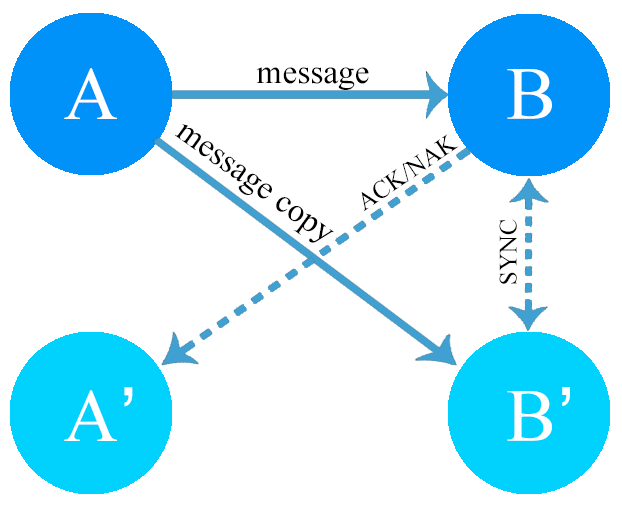
\includegraphics[width=0.7\columnwidth]{Figures/cons_protocol}
%  \end{center}
%  %\vskip -0.25in
%  \caption{Consistency protocol for lsMPI.}
%  \label{fig:cons_protocol}
%\end{figure}

We assume that only MPI operations can introduce non-determinism. MPI\_ANY\_SOURCE receives may result in different message orders between the main and shadow. To deal with this, we always let the main receive a message ahead of the shadow and then forward the message source to its shadow. %(SYNC message in Figure~\ref{fig:cons_protocol}). 
The shadow then issues a receive with the specific source. Other operations, such as MPI\_Wtime() and MPI\_Probe(), can be dealt with by always forwarding the result from the main to the shadow.

%Same as \cite{engelmann2011redundant,ferreira_sc_2011}, consistency protocol introduces runtime overhead due to extra messages. The overhead has been experimentally evaluated to be negligible for most real large-scale applications. Therefore, we believe our protocol, which reduces both message count and bandwidth requirement, should be acceptable. Currently, collectives in lsMPI use linear point-to-point operations internal to lsMPI. We plan to optimize its performance by using binomial tree topology and multi-level hierarchical topology considering hardware locality~\cite{herault2015practical}.

%During normal execution, shadows remain mute, in the sense that 
%all outgoing messages from shadows are suppressed. 
%A shadow process, however, will typically lag behind its main process during execution. Therefore, it is necessary to ensure that the shadow's state is consistent with that of its associated main. %, to successfully complete its associated task in case of failure. 
%To this end, a message-logging protocol is used, % to ensure consistency~\cite{Marz}. These protocols 
%which typically uses a minimum amount of meta-information to store and replicate the non-deterministic decisions~\cite{Marz}. %in the execution of an application.  These meta-data, also called determinants, are exchanged through system-level messages. 

%To provide correct recovery after failure, 
%a mechanism is required to guarantee that every shadow process follows the same computation and communication steps as its main process. 
%After a main fails, its associated shadow will become a new main to recover from this failure. If there are other shadows sharing the same core, they will be terminated and the new main will start consuming the messages in its receiver-side message log at a faster speed. The message logging protocol will ensure that after recovery the new main reaches a consistent state with the rest of the system. 

%Upon failure of a main process, shadow processes will update their address space to ``catch up" with their associated non-failing main processes. A technology, such as remote direct memory access (RDMA), can be used to roll-forward the state of the shadow to be consistent with that of its associated main. Rather than copying data to the buffers of the operating system, RDMA allows to transfer data directly from the main process to its shadow. The zero-copy feature of RDMA considerably reduces latency, thereby enabling fast transfer of data between the main and its shadow.

%Remote Direct Memory Access (RDMA) is used to leap forward the state of the shadow to be consistent with that of its associated main. Rather than copying data to the buffers of the OS, RDMA allows to transfer data directly from the main process to its shadow. The zero-copy feature of RDMA considerably reduces latency, thereby enabling fast transfer of data between the main and its shadow.

 


